\section {Introduction}
In the last 50 years, the experimental exploration of the nucleon structure with electron accelerators has been mainly focused on two classes: measurements of form factors (FFs) through the elastic scattering to obtain the information about the spatial density of nucleons; and measurements of the inclusive deep inelastic process to obtain the parton distribution functions (PDFs) which contain the nucleon's momentum density. Using various experimental techniques, a large group of data with great precision and extensive coverage has provided powerful inputs to understand the mechanism of the hadron structure, and meanwhile, revealed many unsolved puzzles.

In 1990s, a new concept for the description of the nucleon structure was introduced by Mueller, Ji and Radyushkin~\cite{Mueller:1998fv,Ji97-1,Ji97-2,Rad97}, known as the Generalized Parton Distributions (GPDs). GPDs provide a link between electromagnetic form factors and parton distributions~\cite{Die03,Bel05} within the same formalism. What's more, they probe the internal dynamics of the nucleon, e.g. the transverse spatial distribution as a function of the longitudinal momentum fraction of the quarks. One of the important applications is to quantify the angular momentum of quarks contributed to the nucleon spin through the Ji's sum rule~\cite{Ji97-1}.

Deeply Virtual Compton Scattering (DVCS) is the golden channel to experimentally study GPDs~\cite{Bel05}. In electron scattering off nucleons with sufficient large momentum transfer, one measures the hard exclusive photons produced in the Bethe-Heitler (BH) and the DVCS processes as well as their interference, and isolates the DVCS amplitude which is described in terms of GPDs.%With all possible beam and target polarization, the DVCS can give access to and separate the combination of GPDs by measuring the azimuthal dependence of cross sections and asymmetries. 

Several DVCS experiments with proton targets have been carried out in Hall A and Hall B at Jefferson with 6~GeV electron beam. The Hall A experiment~\cite{MunozCamacho:2006hx,Defurne:2015kxq} focused on the precise helicity-dependent and helicity-independent cross section measurements in a limited phase-space. The Hall B experiment used CLAS~\cite{PhysRevLett.100.162002,Jo:2015ema} to measure the beam-spin and target-spin asymmetries and cross sections over a large kinematic range with limited precision. Meanwhile, the HERMES experiments have measured various asymmetries~\cite{Airapetian:2001yk, Airapetian:2012mq, Airapetian:2010ab, Airapetian:2008aa, Airapetian:2011uq, Airapetian:2006zr, Airapetian:2009aa, Airapetian:2009bi} using 27~GeV electron and positron beams on unpolarized, longitudinally polarized and transversely polarized proton targets, but their results suffer from large uncertainties. With the 12~GeV upgrade, several experiments in Hall A and B using CLAS12 have been approved to measure the beam-spin asymmetry and target-spin asymmetry with longitudinally polarized proton target~\cite{halla:e12-06-114,clas12:e12-06-119}. 

The DVCS measurement on neutrons is more difficult mainly due to less production yields, smaller asymmetries and bigger demands on the experimental techniques compared with the proton-DVCS case. The first neutron-DVCS measurement was performed in the E03-106 experiment in Hall A with polarized beam on a deuterium target. This pioneering work established the importance of the neutron-DVCS measurement but was limited to a narrow phase space. An approved CLAS12 experiment~\cite{clas12:e12-11-003} aims to measure the beam-spin asymmetry with unpolarized neutron target. To allow for a fully flavor decomposition to extract the GPDs of individual quarks, it is desired to collect precise neutron data in a more complete phase space and with more experimental observables, especially with the transversely polarized target which is essential to access the GPD $E$. The main goal of this proposal is to perform the first measurement of the DVCS on transversely polarized neutrons with 11~GeV longitudinally polarized electron beam.
\section {Motivation}
\subsection{Generalized Parton Distributions}
The DVCS amplitude can be factorized into two parts in the Bjorken limit: the hard scattering part which can be precisely calculated by perturbative QCD, and the soft part which contains information about the electromagnetic structure of the nucleon, described by a list of Generalized Parton Distributions (GPDs), $H$, $E$, $\tilde H$ and $\tilde E$, where the first two functions, called unpolarized GPDs, correspond with averages of the quark/gluon helicity, and the last two functions involve differences of quark/gluon helicities and hence are called polarized GPDs. In the rest of this proposal, unless specified, we will only discuss the GPDs of quarks in the valence region.

\begin{figure}[!ht]
 \begin{center}
  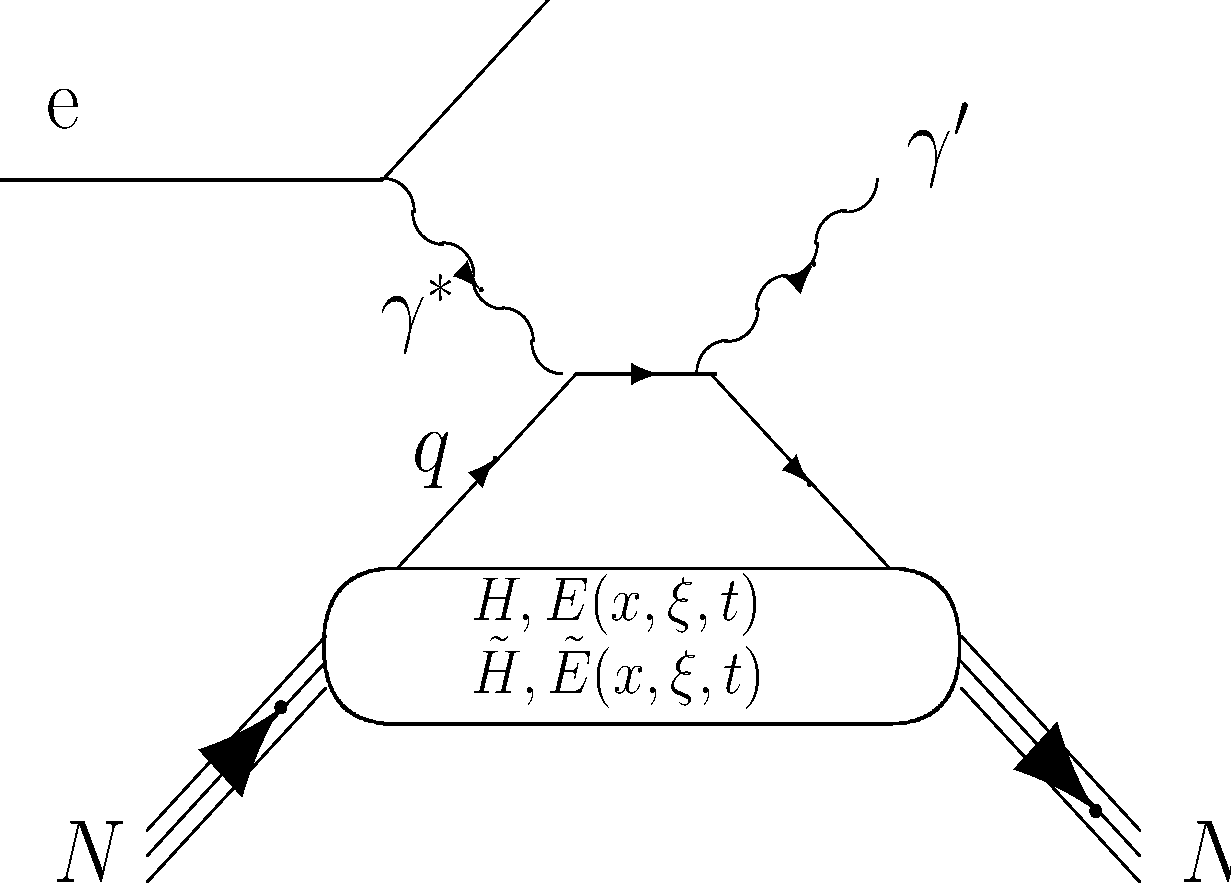
\includegraphics[width=0.4\textwidth]{./figures/dvcs.pdf}
   \caption[Handbag diagram of the DVCS process]{\footnotesize{Handbag diagram of the DVCS process}}
  \label{dvcs_gpd}
 \end{center}
\end{figure}
 As shown in Fig.~\ref{dvcs_gpd}, a highly virtual photon scatters on a quark of which the initial and final momentum fractions are given as $x+\xi$ and $x-\xi$, respectively. The struck quark goes back to its initial nucleon by emitting a real photon so the nucleon remains intact. GPDs are functions of $x$, $\xi$ and $t$, where $x$ denotes the average light-cone momentum fraction of the quark and is not experimentally measurable; $\xi$ represents the longitudinal momentum fraction transferred to the nucleon and in Bjorken limit of infinite $Q^{2}$, it reduces to $\xi=x_{bj}/(2-x_{bj})$, where $x_{bj}$ is the well known DIS variable defined as $x_{bj}=Q^{2}/(2k\cdot k')$ where $k$ and $k'$ are the initial and final four momenta of the electron; $t$ represents the total square momentum transferred to the nucleon, given as $t=\Delta^{2}=(p-p')^{2}$, where $p$ and $p'$ are the four momenta of the nucleon before and after the scattering, respectively. The GPDs also depend on $Q^{2}$ but the variation can be predicted through the evolution equations and doesn't reveal the non-perturbative part of the nucleon. In practice, the $Q^{2}$ dependence is usually dropped out from the expressions.

 The elastic form factors can be given by the first moments of the GPDs~\cite{Gui03}:
\begin{align}
   & \int_{-1}^{+1} dx H^{q}(x,\xi,t)=F_{1}^{q}(t),\\
& \int_{-1}^{+1} dx E^{q}(x,\xi,t)=F_{2}^{q}(t),\\
& \int_{-1}^{+1} dx \tilde H^{q}(x,\xi,t)=G_{A}^{q}(t),\\
& \int_{-1}^{+1} dx \tilde E^{q}(x,\xi,t)=G_{p}^{q}(t),
\end{align}
where $q$ denotes the quark flavor. $F_{1}^{q}(t)$ and $F_{2}^{q}(t)$ are the Dirac and Pauli form factors, $g_{A}^{q}$ and $g_{P}^{q}$ are the axial and pseudoscaler form factors, respectively. The GPDs $H$, $\tilde H$ are linked to the parton distribution functions, $q(x)$ and $\Delta q(x)$ in the forward limit:
\begin{eqnarray}
  H^{q}(x,\xi=0,t=0)&=&q(x), \\
  \tilde H^{q}(x,\xi=0,t=0)&=&\Delta q(x), 
\end{eqnarray}

One of the most important properties of the GPDs is the Ji's sum rule which would give access to the contribution of quark angular momentum to the nucleon's spin:
\begin{equation}
  J^{q}=\frac{1}{2}\Delta\Sigma^{q}+L^{q}=\frac{1}{2}\int_{-1}^{+1}dx x [H^{q}(x,\xi,t=0)+E^{q}(x,\xi,t=0)],
\end{equation}
where $\Delta\Sigma^{q}$  is the contribution of the spin of quarks which was already measured in polarized deep inelastic scattering. Note that the sum rule also applies to the gluon GPDs. Hence the Ji's sum rule provides an experimental way to decompose the nucleon spin in terms of the quark and gluon contributions. Together with measurements of the quark spin in the DIS process, the sum rule will determine the quark orbital angular momentum contribution to the nucleon spin.

In order to study the contribution of the quark orbital angular momentum ($L_{q}$) to the nucleon spin, one needs to determine the $E$ and $H$ GPDs for each quark. However, experimentally, we only measure the GPDs of neutron and proton instead of quarks. Similar to the determination of FFs and PDFs of different quarks, one has to measure both the neutron and proton GPDs and then carry out a flavor separation. For example, in the valance quark region,
\begin{eqnarray}
    H^{p}(\xi,\xi,t)&=&\frac{4}{9}  H^{u}(\xi,\xi,t)+\frac{1}{9}  H^{d}(\xi,\xi,t),\\
    H^{n}(\xi,\xi,t)&=&\frac{1}{9}  H^{u}(\xi,\xi,t)+\frac{4}{9}  H^{d}(\xi,\xi,t),
\end{eqnarray}
form which obtains:
\begin{eqnarray}
    H^{u}(\xi,\xi,t)&=&\frac{9}{15} (4 H^{p}(\xi,\xi,t) - H^{n}(\xi,\xi,t)),\\
    H^{d}(\xi,\xi,t)&=&\frac{9}{15} (4 H^{n}(\xi,\xi,t) - H^{p}(\xi,\xi,t)).
\end{eqnarray}
The same relation holds for $\tilde H$, $E$ and $\tilde E$.

\subsection {Deeply Virtual Compton Scattering}
\begin{figure}[!ht]
 \begin{center}
  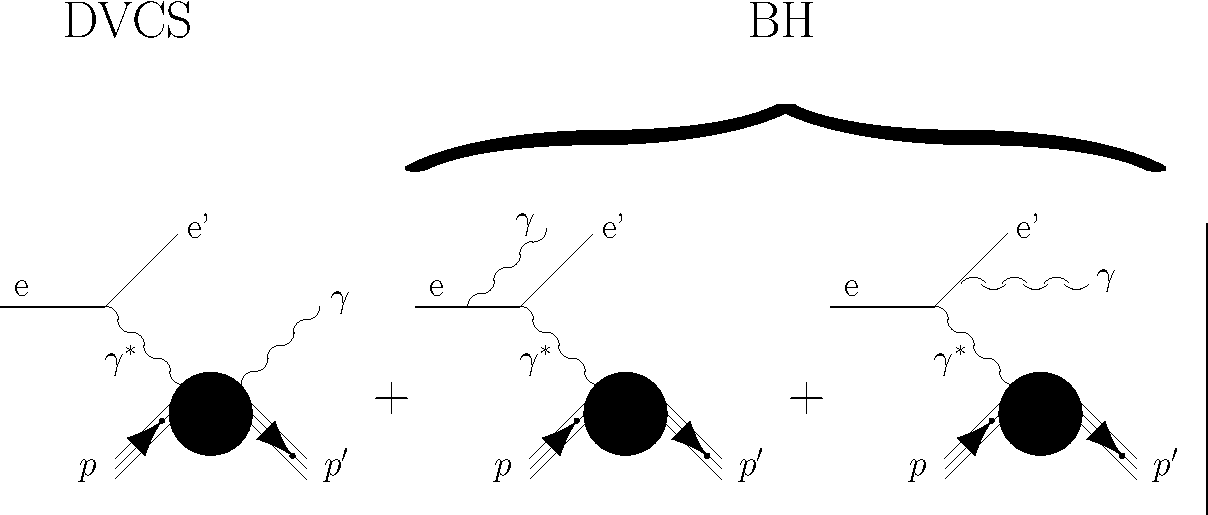
\includegraphics[width=0.6\textwidth]{./figures/bh.pdf}
   \caption[DVCS and Bether-Heitler processes in the $e+N\rightarrow eN\gamma$ reaction]{\footnotesize{DVCS and Bether-Heitler processes in the $e+N\rightarrow eN\gamma$ reaction. The cross section is composed of the amplitudes of these two processes as well as their interference term.}}
  \label{dvcs_bh}
 \end{center}
\end{figure}
The $e+N\rightarrow eN\gamma$ reaction is composed of two processes including the DVCS and the Bethe-Heitler (BH) processes. The later one describes the radiation of the photon by the incoming or scattered electron, as shown in Fig.~\ref{dvcs_bh}. The measure differential cross section of the hard exclusive photon production can be given as the sum of the DVCS, BH processes and their inference:
 \begin{equation}
   \frac{d^{5}\sigma}{dx_{bj}dydtd\phi d\varphi}=\frac{\alpha^{3}x_{bj}y}{16\pi^{2}Q^{2}\sqrt{1+\varepsilon^{2}}}\vert \mathcal{T} \vert^{2}
 \end{equation}
where $\varepsilon=2x_{bj}M/Q$ and $y$ is the fraction of the electron energy lost in the nucleon rest frame. As shown in Fig.~\ref{dvcs_ref}, $\phi$ is the angle between the leptonic plane and the hadronic plane and $\varphi$ is the angle between the polarization vector and the recoil nucleon. The reaction amplitude, $\vert\mathcal{T}\vert^{2}$, can generically be expressed as:
\begin{eqnarray}
 \vert \mathcal{T}\vert^2  = \vert \mathcal{T}_{DVCS}\vert^2 + \vert \mathcal{T}_{BH}\vert^2+ \mathcal{I}, \label{eq:dvcs_amp}\\
\mathcal{I} = \mathcal{T}_{DVCS}^{*}\mathcal{T}_{BH} + \mathcal{T}_{BH}^{*}\mathcal{T}_{DVCS},
\end{eqnarray}
where $\mathcal{T}_{DVCS}$ and $\mathcal{T}_{BH}$ represent the amplitudes of the DVCS and BH processes, and $\mathcal{I}$ denotes their inference term. 
\begin{figure}[!ht]
 \begin{center}
  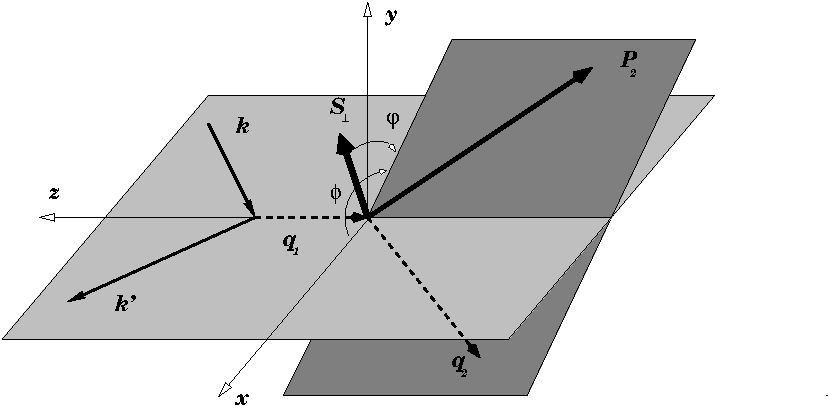
\includegraphics[width=0.6\textwidth]{./figures/refdvcs.pdf}
   \caption[Reference frame of the DVCS process]{\footnotesize{Reference frame of the DVCS process. The reference frame is composed of two planes: the directions of the incoming electron and the scattered electron form the leptonic plane. The directions of the recoil nucleon and the real photon in the final state form the hadronic plane. This plot shows the target in the transversely polarized case where the x and y directions are in and perpendicular to the leptonic plane, respectively.}}
  \label{dvcs_ref}
 \end{center}
\end{figure}
Fig.~\ref{dvcs_ref} illustrates the $e+N\rightarrow eN\gamma$ reaction with relevant kinematic variables.

The DVCS amplitude contains the information about the GPDs with the convolution integral:
\begin{eqnarray}
\mathcal{T}_{DVCS} \propto \int_{-1}^{+1}d x {{H(x,\xi,t)} \over {x - \xi + i \epsilon}}=
{\cal P} \int_{-1}^{+1}d x {H(x,\xi,t) \over {x - \xi}} -i\pi H(\xi,\xi,t) ,
\label{eq:imredecomp}
\end{eqnarray}
where ${\cal P}$ denotes the principal value integral. Eq.~(\ref{eq:imredecomp}) can be decomposed into a real and an imaginary part, and including other GPDs $E$, $\tilde{H}$ or $\tilde{E}$, there are eight GPD-related quantities that can be extracted from the DVCS process~\cite{Gui03}:
\begin{eqnarray}
H_{Re}(\xi , t) &\equiv& {\cal P} \int_0^1 d x \left[ H(x, \xi, t) - H(-x, \xi, t) \right] C^+(x, \xi),\label{eq:eighta} \\
H_{Im}(\xi , t) &\equiv& H(\xi , \xi, t) - H(- \xi, \xi, t),\label{eq:eightb} \\
E_{Re}(\xi , t) &\equiv&   {\cal P}  \int_0^1 d x \left[ E(x, \xi, t) - E(-x, \xi, t) \right] C^+(x, \xi),\label{eq:eightc} \\
E_{Im}(\xi , t) &\equiv& E(\xi , \xi, t) - E(- \xi, \xi, t), \label{eq:eightd} \\
\tilde H_{Re}(\xi , t) &\equiv&  {\cal P}  \int_0^1 d x \left[ \tilde H(x, \xi, t) + \tilde H(-x, \xi, t) \right] C^-(x,\xi),\label{eq:eighte} \\
\tilde H_{Im}(\xi , t) &\equiv& \tilde H(\xi , \xi, t) + \tilde H(- \xi, \xi, t),\label{eq:eightf} \\
\tilde E_{Re}(\xi , t) &\equiv&  {\cal P}  \int_0^1 d x \left[ \tilde E(x, \xi, t) + \tilde E(-x, \xi, t) \right] C^-(x,\xi),\label{eq:eightg} \\
\tilde E_{Im}(\xi , t) &\equiv& \tilde E(\xi , \xi, t) + \tilde E(- \xi, \xi, t), \label{eq:eighth} 
\end{eqnarray}
with the coefficient functions $C^\pm$ defined as~:
\begin{equation}
C^\pm(x, \xi) = \frac{1}{x - \xi} \pm \frac{1}{x + \xi}
\end{equation}
\noindent
Note that one has reduced the $x$-range of integration from $\{-1,1\}$ to $\{0,1\}$ in the convolutions. Eq.~\ref{eq:eighta} through Eq.~\ref{eq:eighth} are refer to as the Compton form factors (CFFs). For convenience, four complex functions are introduced:
\begin{eqnarray}
{\cal H}(\xi,t) &\equiv& H_{Re}(\xi,t) - i \pi H_{Im}(\xi,t),
\label{eq:cffcomplex-1} \\
\tilde{\cal H}(\xi,t) &\equiv& \tilde H_{Re}(\xi,t) - i \pi \tilde H_{Im}(\xi,t),
\label{eq:cffcomplex-2} \\
{\cal E}(\xi,t) &\equiv& E_{Re}(\xi,t) - i \pi E_{Im}(\xi,t),
\label{eq:cffcomplex-3} \\
\tilde{\cal E}(\xi,t) &\equiv& \tilde E_{Re}(\xi,t) - i \pi \tilde E_{Im}(\xi,t).
\label{eq:cffcomplex-4}
\end{eqnarray} 

On the other hand, the BH amplitude can be precisely calculated theoretically with the well measured $F_{1}$ and $F_{2}$ form factors. The BH cross section strongly depends on the kinematic variables, $Q^{2}$, $x_{bj}$, $t$ or $\phi$. One of the distinct features is a sharply enhancement around $\phi=0$ or $\phi=180$ which corresponds to the regions where the radiated photon is along the directions of the incoming electron or the scattered one, respectively. The BH amplitude varies significantly over the entire phase space and it can be either overwhelming or can be ignored when compared with the DVCS amplitude. One can look for unique experimental observables that are sensitive to the $\cal{I}$ term, such that the linear combination of CFFs can be directly accessed via the DVCS amplitude while the BH amplitude thereupon serves as an asset.

\subsection {Experimental Observable}
 Taking into account the fact that the four GPDs reflect different combination of the nucleon spin and quark helicities, one is sensitive to different combinations of them by measuring various experimental quantities with different beam and target polarization. For example, one can measure DVCS with different beam- and/or target-spin polarizations as the cross section differences give access to the interference term (${\cal I}$) of the BH and DVCS processes~\cite{Belitsky:2001ns, Gui03}:
 \begin{eqnarray}
  \Delta\sigma_{LU} &\propto& \sin\phi \;\; Im\{F_{1}{\cal H}+\xi(F_{1}+F_{2}) \tilde {\cal H}-kF_{2}{\cal E}+...\}, \label{eq:kirch1} \\
  \Delta\sigma_{UL} &\propto& \sin\phi \;\; Im\left\{F_{1}\tilde{\cal H}+\xi(F_{1}+F_{2})\left(\tilde{\cal H}+\frac{x_{bj}}{2}{\cal E}\right)-\xi kF_{2}\tilde{\cal E}+...\right\}, \label{eq:kirch2} \\
  \Delta\sigma_{LL} &\propto& (A+B\cos\phi) \;\;Re\left\{F_{1}\tilde{\cal H}+\xi(F_{1}+F_{2})\left({\cal H}+\frac{x_{bj}}{2}{\cal E}\right)+...\right\}, \label{eq:kirch3}\\
  \Delta\sigma_{UTx} &\propto& \sin\phi \;\; Im\{k(F_{2}{\cal H} -F_{1} {\cal E})+...\},  \label{eq:kirch4} \\
  \Delta\sigma_{LTx} &\propto& (A+B\cos\phi) \;\;Re\left\{k(F_{2}{\cal H} -F_{1} {\cal E})+...\right\}, \label{eq:kirch5}
%  \\
%  \Delta\sigma_{UTy} &\propto& \sin\phi \;\; Im\{X...\},  \label{eq:kirch6} \\
 % \Delta\sigma_{LTy} &\propto& (A+B\cos\phi) \;\;Re\left\{X...\right\}, \label{eq:kirch7}
 \end{eqnarray}
where $\Delta\sigma$ stands for a cross section difference at certain beam (first subscript) and target (second subscript) polarization directions (``$U$" for unpolarized, ``$L$" for longitudinally polarized, and ``$Tx$" or ``$Ty$" for transversely polarized in ($x$) or perpendicular ($y$) to the leptonic plane as shown in Fig.~\ref{dvcs_ref}). Furthermore, $F_{1}$ and $F_{2}$ are the Dirac and Pauli form factors, and the kinematic variable $k$ is defined as~: $k= -t / (4m_N^2)$. The detailed correlations between the cross sections and the DVCS+BH amplitudes have been worked out in Ref.~\cite{Belitsky:2001ns}.

From Eq.~\ref{eq:kirch1} to Eq.~\ref{eq:kirch5}, each cross section difference is only sensitive to certain CFFs when neglecting terms multiplied by kinematic factors with small values, such as $\xi$, $x_{B}$ or $k$. For example, among these proton CFFs,  $Im\{{\cal H}^{p}\}$ dominates in $\Delta\sigma_{LU}$ and instead, $Im\{\tilde {\cal H}^{p}\}$ is the largest contribution to $\Delta\sigma_{UL}$. One also notices that the observables with single-spin polarization access the imagine parts of the CFFs while the double-spin polarization terms probe the real parts. The sensitivity of these observables to the neutron CFFs changes due to different FFs values, e.g. $F^{n}_{1}\approx 0$ when $t$ is small.

During the experiments it is simpler to measure the asymmetries with various beam and target polarization to avoid the normalization issue, even though the sensitivity to the CFFs is not as direct as the one from the cross section difference. %In Table~\ref{table:cff_asym}, we summarize the proton and neutron CFFs that the asymmetries are sensitive to with different beam and target polarization. 
% \begin{table}\centering
% \begin{tabular}{|c|c|c|}
% \hline
% {\bf Polarization}       &   {\bf Asymmetry}  & {\bf Compton Form Factors} \\\hline 
% Long. Polarized Beam     & $A_{LU}$  & $Im\{ \mathcal{H}^{p},\tilde{\mathcal{H}}^{p}, \mathcal{E}^{p} \}$, \\  
% Unpolarized Target       &           & $Im\{ \mathcal{H}^{n},\tilde{\mathcal{H}}^{n}, \mathcal{E}^{n} \}$ \\\hline 
% 
% Unpolarized Beam         & $A_{UL}$  & $Im\{ \mathcal{H}^{p},\tilde{\mathcal{H}}^{p} \}$, \\  
% Long. Polarized Target   &           & $Im\{ \mathcal{H}^{n}, \mathcal{E}^{n} ,\tilde{\mathcal{E}}^{n}\}$ \\\hline 
% 
% Long. Polarized Beam     & $A_{LL}$  & $Re\{ \mathcal{H}^{p},\tilde{\mathcal{H}}^{p} \}$, \\  
% Long. Polarized Target   &           & $Re\{ \mathcal{H}^{n}, \mathcal{E}^{n} ,\tilde{\mathcal{E}}^{n}\}$ \\\hline 
% 
% Unpolarized Beam         & $A_{UT}$  & $Im\{ \mathcal{H}^{p},\mathcal{E}^{p} \}$, \\  
% Trans. Polarized Target  &           & $Im\{ \mathcal{H}^{n} \}$ \\\hline 
% 
% Long. Polarized Beam     & $A_{LT}$  & $Re\{ \mathcal{H}^{p},\mathcal{E}^{p} \}$, \\  
% Trans. Polarized Target  &           & $Re\{ \mathcal{H}^{n} \}$ \\\hline 
% \end{tabular}
% \caption{\footnotesize{Asymmetries with different beam and target polarization and corresponding Compton form factors of protons and neutrons~\cite{Belitsky:2001ns,Gui03} .}}\label{table:cff_asym}
% \end{table} 
